\chapter{Teoria sugli algoritmi}

\section{Space Rank}
Una buona conoscienza delle abitudini degli utenti, mediante i loro spostamente,
\`e di fondamentale importanza per poter sviluppare algoritmi di previsioni della
destinazione. Infatti i luoghi di maggior interesse risulteranno essere le destinazioni
dei loro spostamenti. Tuttavia, in questo particolare contesto, le definizioni del
concetto di importanza e dei relativi indici di valutazione compongono un campo di
ricerca di notevole interesse.\\
In questa sezione viene proposta una metodologia di analisi dei dati volta
a stimare l'importanza delle localit\`a sulla base dei comportamenti degli utenti.
Mediante i dati relativi inerenti alle visite effettuare degli utenti nelle singole
localit\`a, ci si pone l'obiettivo di ottenere dei valori rappresentati l'importanza
che ogni localit\`a assume nelle abitudini degli utenti.

\subsection{Criteri di valutazione dell'importanza}
Nella letteratura possiamo trovare diversi casi in cui risulta necessario lo sviluppo
di sistemi di valutazione dell'importanza delle localit\`a come in in \cite{cit_42},
nel quale viene presentato l'algoritmo \textbf{Predestination}, che esegue
una suddivisione del territorio ed una valutazione dell'importanza di ciascuna
sezione, per indicarne l'interesse per utente esaminato.
Un altro esempio di particolare interesse \`e inoltre l'articolo \cite{cit_43},
nel quale si propone un modello gravitazionale atto a considerare i
flussi di una citt\`a per decidere in quali zone sia preferibile andare ad aprire
nuove attivit\`a commerciali. Questi esempi ci fanno capire quanto sia importate
la scelta di un appropriato criterio di valutazione di importanza delle regiorni.
Definire quali siano le localit\`a importanti per un utente non e tuttavia semplice.
Alcuni studi \cite{cit_44} hanno dimostrato che le probabilit\`a che ciascuno di
noi si trovi in una certa localit\`a sono legate alla legge di potenza,
ovvero che tali probabilit\`a relativamente ad una localit\`a sono proporzionali
all'inverso della posizione occupata dalla localit\`a stessa in una scala di importanza.
Questo ci fa dedurre che esiste un ordinamento delle localit\`a basato sull'importanza
che le localit\`a hanno per ognuno di noi. Esaminando \cite{cite_44} possiamo inoltre
dedurre, dato che le persone frequantano abbitualmente gli stessi luoghi, che analizzando
i comportamenti passati dell'utente possiamo definire un elenco ordinato di zone di
interesse in modo tale da prevedere i suoi movimenti.Per definire l'importanza
che ciascuna localit\`a ha per l'utente, e dunque intuitivo adottare i seguenti indici:
\begin{itemize}
\item $\sharp$\textit{visits}: il numero di volte in cui l'utente \`e stato nella localit\`a;
\item \textit{avgTime}: il tempo medio delle visite effettuate dall'utente nella localit\`a;
\item \textit{totTime}: il tempo totale passato dall'utente nella localit\`a durante le sue visite.
\end{itemize}
Questi indici sono facilmente calcolabili da una qualsiasi collezione (previa
standardizzazione della struttura del contenuto) ma, considetati singolarmente,
possono dare solo una visione parziale delle abitudini degli utenti, e per alcune
applicazioni non sarebbero sufficenti. Se valutiamo singolarmente gli indici notiamo che:
\begin{itemize}
\item $\sharp$\textit{visits} equipara le localit\`a di passaggio con quelle in avvieneuna lunga sosta;
\item \textit{avgTime} equipara localit\`a frequentemente visitate a quelle che vengono raramente raggiunte;
\item \textit{totTime} equipara sia le lughe soste che l'alto numero di passaggio su una particolare cella.
\end{itemize}
Migliore dunque sembrerebbe l'utilizzo dell'indice \textit{totTime}, in quanto esso riesce a valorizzare
sia le lunghe permanenze che un alto numero di passaggi ma rimane per\`o comunque
il problema di come riuscire a differenziare le celle con stesso \textit{totTime}.
Per questo si \`e deciso di introdurre un indice derivato, definito come \textit{combLinear},
composto dalla combinazione linere degli indici $\sharp$\textit{visits} ed \textit{totTime}.
Questa soluzione da la possiblit\`a di differenziare le celle che hanno lo stesso valore ma
porta di problema di come pesare i due indici durante il calcolo della combinazione lineare.\\

Dopo aver definto diverse proposte per la rilevazione dell'importanza delle localit\`a,
ognuna con pregi e difetti, risulta interessante comparate, insieme agli algoritmi di
previsione di traiettorie basati sulle pesauta delle localit\`, un nuovo indice basato su
una pi\`u complessa valutazione dei dati ma simile ai precedente per risultati.
Nella ricerca di una migliore valutazione delle localit\`a ci si \`e imbattuiti nell'algoritmo
di PageRank \cite{cit_45}, utilizzato dai motori di ricerca per la catalogazione e
l'ordinamento dei documenti ipertestuali. Tale algoritmo, mediante un grafo ottenuto dalla
mappatura dei collegamenti ippertestuali tra pagine web, stima l'importanza dei documenti
considerati. Si \`e dunque deciso di sviluppare il concetto proposto dall'algoritmo PageRank
per sviluppare il nuovo indice \textit{SpaceRank} che, mediante il grafo ottenuto
dagli spostamenti dell'utente, stimer\`a l'importanza delle localit\`a di interesse dell'utente.

\subsection{PageRank}
L'algoritmo di PageRank \cite{cit_45} ha avuto origine nel 1995 da un progetto di ricerca
della Stanford University, a cura di Larry Page. Quest'ultimo, insieme a Sergey Brin,
svilupparono un motore di ricerca basata proprio sul questo algoritmo che negli anni a verire
divenne il motore di ricerca pi\`u utilizzato, Google. Basato sull'idea di misurare
l'importanza di ciascun elemento di un insieme di documenti con collegamenti ipertestuali
mediante un valore numerico rappresentante la probabilit\`a che una persona arrivi
a quel dato documento scegliendo ciclicamente a caso uno dei collegamenti presenti
nel documento ipertestuale che sta leggendo. Il processo matematico, utilizzato per
il calcolo di tale valore per a ciascuno dei documenti, si basa sulle catene di Markov.
Prendendo in considerazione l'insieme dei documenti ipertestuali, viene calcolata la matrice
matrice \textit{n x n}, dove n \`e il numero dei documenti presenti nell'insieme.
Su ciascuna riga vengono inseriti i valori relativi ai collegamenti ipertestuali
che puntano a ciascuno dei documenti indicati dalle colonne. Sulla matrice ottenuta viene
effettuata una normalizzazione tale da rendere la somma dei valori di ciascuna riga pari ad 1
ottenendo la matrice di adiacenza del grafo delle citazioni dell'insieme di documenti.
La matrice risultante pu\`o essere interpretata come una catena di Markov ed il calcolo
dell'autovettore dominante della matrice di adiacenza definisce la probabilit\`a di
trovarsi in ciascuno degli stati della catena di Markov durante una camminata casuale,
ovvero la probabilit\`a di raggiungere ciascuno dei documenti scegliendo ciclicamente
a caso uno dei collegamenti ipertestuali contenuti nei documenti che vengono presentati,
ovvero il valore di PageRank.\\
Tuttavia questo calcolo non \`e esente da problemi \cite{cit_49}.
Il primo problema \`e relativo alla catena di Markov, la quale potrebbe non essere ergodica.
Una catena di Markov si definisce ergodica se ciascuno stato della catena (ovvero ciascun nodo del grafo) \`e:
\begin{itemize}
\item aperiodico: se il suo periodo \`e pari a 1, ovvero se lo stato non deve sempre
occorrere dopo un multiplo di un certo numero di passi;
\item ricorrente positivo: se in una camminata casuale infinita c'\`e sempre
probabilit\`a di ritornare in uno stato gi\`a visitato in un numero finito
di passi.
\end{itemize}
Il calcolo dell'autovettore dominante di una matrice relativa ad una catena di
Markov non ergodica potrebbe non convergere e non si avrebbe, quindi, un
limite stabile da poter utilizzare come valore di PageRank.\\
Il secondo problema, invece, riguarda prpprio il concettu su cui si basa questa
metodologia. \`E difficile pensare che utente sfogli un insieme di documenti
seguendo solamente i collegamenti ipertestuali senza mai abbandonare un documento
per uno qualsiasi dei documenti dell'insieme.
Entrambi i problemi descritti possono essere risolti mediante l'utilizzo di
quella che viene comunemente definita matrice di teletrasporto. Quest'ultima
\`e una matrice \textit{n x n} che definisce un grafo con un arco di pari peso tra ciascuna
coppia di nodi. Tale grafo pu\`o essere interpretato come una catena di Markov
in cui ad ogni passo \`e possibile passare dallo stato attuale ad uno qualsiasi
degli stati della catena (compreso quello attuale). Mediante la combinazione lineare
delle normalizzazioni delle due matrici descritte si ottiene la matrice il cui
autovettore dominante contiene i valori di PageRank utilizzati come stima
dell'importanza dei documenti dell'insieme. Per tale combinazione lineare viene
utilizzato un fattore d, comunemente definito fattore di salto, che definisce la
probabilit\`a, stabilita a priori, che l'utente effettui un salto dal
documento in cui si trova ad uno qualsiasi dei documenti dell'insieme, ovvero
di seguire i collegamenti definiti dalla matrice di teletrasporto. Dunque, la
matrice utilizzata per il calcolo dei valori di PageRank sar\`a:
\begin{equation}
P = (1 - d) x A + d x T
\end{equation}
dove A \`e la matrice di adiacenza normalizzata del grafo delle citazioni, T \`e
la matrice di teletrasporto normalizzata e d \`e il fattore di salto. Per il calcolo
dell'importanza delle pagine web, dai motori di ricerca viene solitamente
utilizzato un fattore di salto pari a 0.15.\\
La matrice di PageRank \textit{P} ottenutuna pu\`o essere utilizzarla per calcolare
la matrice di Importanza $M_{imp}$ utilizzando il metodo delle potenze per
ricavarne l'autovettore dominante. Sia x vettore qualsiasi di dimensione n,
e \textit{P} la matrice di PageRank otterremo la matrice $M_{imp}$ come segue:
\begin{equation}
M_{imp} = \lim_{k \rightarrow +\infty} x P^{k}
\end{equation}
La formulazione proposta in realt\`a non viene mai implementata in quanto
presenta problemi di overflow ed underflow. Per evitarli \`e necessario
eseguire ad ogni passo una normalizzazione del vettore ottenuto, costruendo
una successione definita come segue:
\begin{equation}
\left\{\begin{matrix}
M_{aux}(i+1) = M_{imp}(i)P
\\ \beta_{i+1} = normaDue[M_{aux}(i+1)]
\\ M_{imp}(i+1) = \frac{M_{aux}(i+1)}{\beta_{i+1}}
\end{matrix}\right.
\end{equation}
che termina non appena $ M_{imp}(n) - M_{imp}(n- 1) < \varepsilon $ con $ \varepsilon $ scelto dall'utente,
lasciando quindi $ M_{imp} = M_{imp}(n) $.

\subsection{SpaceRank}
In questo capitolo viene proposta, dopo una breve introduzione concettuale, l'analisi
del comportamente dell'algoritmo SpaceRank \cite{cit_49} che, come l'algoritmo di
PageRank da cui trae ispirazione, ha come obiettivo la ricerca dei valori di importanza
delle localit\`a, calcolate mediante l'autovettore delle matrice ottenuta dall'agoritmo.

\subsubsection{Formalizzazione del problema}
L'obbiettivo di questo algoritmo \`e, dato un insieme di informazioni relative all'ubicazione
di un insieme di utenti in una data area e lungo un dato periodo di tempo, di stimare
l'importanza delle localit\`a dell'area di interesse basate sulle informazione dell'insieme.
Queste localit\`a di interesse sono un insieme di sotto-aree $L = l_{0},l_{1},\dots,l_{n-1}$
ottenute della divisione dell'area di interesse totale. Tali localit\`a potrebbero
avere forme e dimensioni differenti, ma per semplicit\`a, in questa discussione
supporremo che abbiamo forma e dimensioni identiche. In Figura 1.1 sono rappresentati
alcuni esempi grafici delle localit\`a sopra descritti.\\
Definiamo $N_{i}$ come l'insieme di tutte le localit\`a vicine ad $l_{i}$, ovvero l'insieme
di tutte le localit\`a raggiungibili da $l_{i}$ con un solo passaggio, compresa $l_{i}$ stessa,
ed N come l'insieme di tutti gli insiemi $N_{i}$. Disponendo dei dati relativi
agli spostamenti, quindi dell'ubicazione e della velocit\`a, di uno o pi\`u utenti
durante un periodo di tempo possiamo, per ciascun utente, creare un registro
storico $R_{u} = r_{0},r_{1},r_{2},\dots$. Ogni elemento dell'insieme \`e una tripla
$r_{i} = (t,l,s)$dove t \`e un riferimento temporale relativo all'istante in cui \`e
stata effettuata la campionatura, $l \in L$ \`e la localita registrata ed s \`e
la velocit\`a di spostamento dell'utente in quell'istante. Definiamo quindi $R = R_{0},R_{1},\dots,R_{n}$
l'insieme dei registri relativi agli n utenti del campione. Dati gli insiemi $L, N$ ed $R$, l'obiettivo \`e quello di ottenere
un valore numerico che stimi l'importanza di ciascuna localit\`a $l \in L$.

\begin{figure}
  \centering
  \begin{subfigure}[a]{0.3\textwidth}
      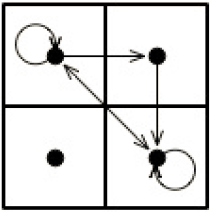
\includegraphics[scale=0.4]{grafo_1.png}
      \label{fig:a}
  \end{subfigure}
  \begin{subfigure}[b]{0.3\textwidth}
      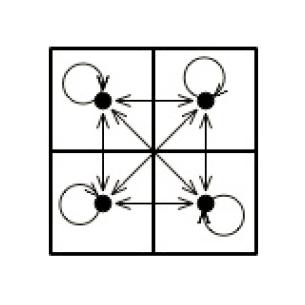
\includegraphics[scale=0.4]{grafo_2.png}
      \label{fig:a}
  \end{subfigure}
  \begin{subfigure}[c]{0.3\textwidth}
      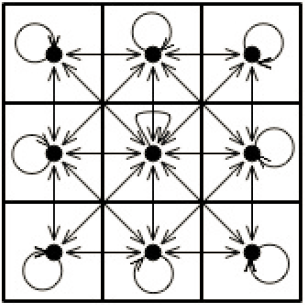
\includegraphics[scale=0.4]{grafo_3.png}
      \label{fig:a}
  \end{subfigure}
  \caption[Fig 1.1]{Esempi di grafi delle localit\`a}
  \label{fig2.1}
\end{figure}

\subsubsection{Matrice basata sul registro storico dei dati}
Come prima procedura, l'algoritmo SpaceRank prevede la mappatura
dei registri relativi alla campionatura dell'ubicazione degli utenti in un grafo
pesato diretto, rappresentante le abitudini degli utenti osservati.
Sia A la matrice di adiacenza $n x n$ (dove n \`e la cardinalit\`a di L) del
grafo delle abitudini, inizialmente nulla (cio\`e $A[i, j] = 0$ per ogni di i e j
compresi tra 0 ed n-1). Dato l'insieme R, per ciascun $R_{u} \in R$, per ciascuna
coppia di elementi di $R_{u}$ temporalmente successivi $r_{x}$ ed $r_{x+1}$, deve essere eseguito
l'aggiornamento $A[i, j] = A[i, j] + 1$, dove $l_{i}$ \`e la localit\`a indicata dalla
tripla $r_{x}$ ed $l_{j}$ \`e la localit\`a indicata dalla tripla $r_{x+1}$.
Dopo aver mappato tutti gli spostamenti, ogni elemento $A[i, j]$ della matrice A
conterr\`a il numero di movimenti (ovvero passaggi da una localit\`a ad un'altra)
dalla localit\`a i alla localit\`a j effettuati dagli utenti durante il periodo di osservazione.
\`E da notate che se l'utente non compia uno spostamente di locali\`a durante 2 campionamenti
temporalmente successivi, questo spostamenteo verr\`a mappato come un ciclo sullo
stesso nodo del grafo. Definiremo questo spostamente come permaneza.\\
\\
Quanto descritto appena descritto \`e visibile mediante di grafici in Figura 2.1.
Vengono vuisualizzate le divisione in localit\`a di un'area di interesse con
relativi archi (nella figura non sono visibili i pesi assegnati agli archi) rappresentanti
gli spostamenti. Per ogni immagine di pu\`o notare che nella localit\`a in alto a
sinistra si pu\`o vedere un caso di permanenza.
Tramite un processo di normalizzazione delle righe della matrice A \`e possibile
ottenere una matrice $\bar{A}$, in cui la somma dei valori di una singola riga sia 1.
Ciascun valore $\bar{A}[i, j]$ contenuto in tale matrice pu\`o essere interpretato come
la probabilit\`a che l'utente effettui un movimento dalla localit\`a i alla localit\`a
j sulla base delle abitudini osservate, contenute nell'insieme dei registri R.
Per normalizzare i valori si pu\`o dividere ciascun elemento di ciascuna riga della
matrice per la somma dei valori della riga a cui esso appartiene. Questo \`e uno
dei molti procedimenti possibili, ma anche uno dei pi\`u veloci.

\subsubsection{Matrice di transizione}
La matrice $\bar{A}$ finora ottenuta non \`e utilizzabie per ottenere una soluzione
corretta in quanto si avrebbe una probabilit\`a pari a zero di raggiungere una localit\`a mai visitata
prima dall'utente e la catena di Markov relativa al grafo delle abitudini potrebbe
non essere ergodica. A tal fine pu\`o essere creata una matrice $\bar{B}$,
che definiremo come matrice di transizione, che rappresenti un grafo avente
un nodo per ciascuna localit\`a $l \in L$ ed un arco per ciascuna coppia di localit\`a
contigue. Sia dunque $\bar{B}$ la matrice definita come:

\begin{equation}
\bar{B}[i,j] =
\left\{\begin{matrix}
\frac{1}{c_{i}} & se l_{j} \in N_{i}\\
0 & altrimenti
\end{matrix}\right.
\end{equation}

dove $c_{i}$ \`e la cardinalit\`a dell'insieme $N_{i}$. Tale matrice \`e gi\`a normalizzata e
descrive un grafo corrispondente ad una catena di Markov ergodica in cui si
ha la stessa probabilit\`a di effettuare ad ogni passo una transizione dallo stato
attuale ad uno qualsiasi degli stati che rappresentano le localit\`a vicine a quella
in cui si trova l'utente (compresa quest'ultima).
Ad esempio in Figura 2.1 (b) viene illustrato il grafo di una possibile matrice
$\bar{B}$ relativa ad una area suddivisa in quattro localit\`a disposte in una griglia
$2 x 2$ (nella figura non sono visibili i pesi assegnati agli archi). In questo caso
particolare, l'insieme dei vicini di ciascuna localit\`a comprende tutte le localit\`a
dell'area di interesse. Lo stesso vale per la localit\`a centrale in Figura 2.1 (c),
dove viene illustrato il grafo di una possibile matrice $\bar{B}$ relativa ad un area
suddivisa in nove localit\`a disposte in una griglia $3 x 3$ (nella figura non sono
visibili i pesi assegnati agli archi), ma non per le altre localit\`a di questo secondo
esempio, dalle quali \`e possibile raggiungere solo alcune localit\`a (4 o 6 a seconda
della posizione).

\subsubsection{Combinazioni delle matrici}
Dopo aver ottenuto le due matrici $\bar{A}$ e $\bar{B}$ rappresentanti rispettivamente
le abitudini osservate degli utenti e la conformazione dell'area d'interesse,
possiamo combinare le due matrici per ottenere una matrice normalizzata a cui applicare
il calcolo dell'autovettore dominante. Nel calcolo del PageRank viene definito il fattore
di combinazione d che, in questo contesto, possiamo definire come fattore di
comportamento non abitudinario, dato che definisce la percentuale di probabilit\`a
con cui deve essere presa in considerazione la possibilit\`a che l'utente
si muova al di fuori delle abitudini osservate. La matrice a cui verr\`a dunque
applicato il calcolo dell'autovettore dominante sar\`a:
$$
S = (1 - d) x \bar{A} + d x \bar{B}
$$
Come avviene nel calcolo del PageRank, viene impostato d = 0.15. Un valore minore
darebbe maggiore importanza alle abitudini osservate, mentre un valore superiore
porterebbe in considerazione un comportamento generico e non legato alle abitudini
osservate. I due casi estremi porterebbero a $S = \bar{A}$, con $d = 0$,
ed a $S = \bar{B}$, con $d = 1$. Ovviamente questi ultimi due casi sono da
escludere: il primo perch\'e porterebbe agli stessi problemi a causa dei quali \`e
stata introdotta nel calcolo la matrice $\bar{B}$; il secondo perch\'e non darebbe
alcuna effettiva informazione relativa ai comportamenti osservati degli utenti.

\subsubsection{Calcolo della Matrice di Importanza}
Una volta calcolata la matrice di SpaceRank S, non rimane che utilizzarla per
calcolare la matrice di Importanza $M_{imp}$ utilizzando il metodo delle potenze
per ricavare l'autovettore dominante.\\
Sia x vettore qualsiasi di dimensione n, ed $S$ la matrice di SpaceRank otterremo
la matrice $M_{imp}$ come segue:
\begin{equation}
M_{imp} = \lim_{k \rightarrow +\infty} x S^{k}
\end{equation}
Ovviamente per calcolare effettivamente $M_{imp}$ sara sufficiente eseguire la seguente
successione libera da problemi di underflow ed overflow:
\begin{equation}
\left\{\begin{matrix}
M_{aux}(i+1) = M_{imp}(i)S
\\ \beta_{i+1} = normaDue[M_{aux}(i+1)]
\\ M_{imp}(i+1) = \frac{M_{aux}(i+1)}{\beta_{i+1}}
\end{matrix}\right.
\end{equation}
che termina non appena $ M_{imp}(n) - M_{imp}(n- 1) < \varepsilon $ con $ \varepsilon $ scelto dall'utente,
lasciando quindi $ M_{imp} = M_{imp}(n) $.

\section{ARDA}
Come esposto nell'introduzione, negli ultimi anni sono stati sviluppati diversi
algoritmi per la previsione delle traiettorie degli utenti basati su complicati
modelli matematici e statistici basati su informazioni raccolte nel passato. In
questo capitolo, dopo una breve formalizzazione del problema della previsione
delle traiettorie, viene proposto un modello astratto presentato in \cite{cit_49}
basato sull'utilizzo di un semplice modello fisico dei campi elettrici.

\subsection{Formalizzazione del problema}
Si prenda ad esempio un generico oggetto in movimento su una superficie
bidimensionale. Possiamo indicare tale oggetto generico come oggetto della previsione
(ODP). L'obiettivo \`e quello di determinare la probabilit\`a con cui l'ODP,
che all'istante $t_{0}$ \`e posizionato nel punto $(x_{0}, y_{0})$ sulla superficie,
si potr\`a trovare in ciascuno dei punti del piano ad un certo istante $t_{i}$ nel futuro,
dato un suo attuale vettore di spostamento $\vec{v_{0}}$.
In prima istanza, questo equivale a cercare una funzione a sette parametri:
\begin{equation}
p(x_{0},y_{0},t_{0},\vec{v_{0}},t_{i},x,y)
\end{equation}
che calcoli un valore di probabilit\`a per ciascun punto $(x, y)$ del piano.
Come gi\`a fatto notare, gli spostamenti delle persone non sono puramente casauli,
ma dettati dal'interesse di esse verso un piccolo insieme di luoghi \cite{cit_44}.
Proprio questi luoghi possono esercitare un'attrazione dell'ODP nei suoi spostamenti
visto l'influenza che essi anno nelle storico fornito dell'utente.
Da questo possiamo ricavare una funzione del tipo:
\begin{equation}
p[k_{1},\dots,k_{n}](x_{0},y_{0},t_{0},\vec{v_{0}},t_{i},x,y)
\end{equation}
che calcoli la probabilit\`a che (x, y) sia la posizione dell'ODP al tempo $t_{i}$,
dato uno schema fissato di punti di interesse sulla superficie $[k_{1},\dots,k_{n}]$.

\subsection{Modello astratto di previsione}
Le metafore legate al mondo reale sono largamente utilizzate in diversi campi
dell'informatica. In questo capitolo viene presentato un modello astratto,
per la previsione delle traiettorie degli utenti sfruttando una
metafora legata alla fisica dei campi elettrici.

\subsubsection{Modello gravitazionale}
Un recente studio \cite{cit_44} ha confermato che qualunque persona \`e legata ad un
insieme di luoghi che possiamo definite importanti. Le analisi condotte
indicano che vi sono alte probabilit\`a che in un qualsiasi momento una data
persona si trovi in due o tre localit\`a importanti e basse probabilit\`a che si trovi
in un qualsiasi altro posto. Da queste considerazioni si pu\`o dedurre che se un
utente \`e in movimento ci sono alte probabilit\`a che si stia dirigendo verso uno
di questi punti di interesse. Infatti un gran numero di persone compiono gli stessi
tragitti per arrivare a delle localit\`a importanti (sia per abitudine o per necessit\`a)
Tuttavia, durante la giornata effettuiamo anche altri spostamenti che ci portano in
localit\`a non appartenenti a quel piccolo insieme definite importanti. In questi casi
la probabilit\`a che la destinazione si un nostro persorso sia una di queste localit\`a
meno importanti \`e bassa, ma non nulla.\\
Anche la velocit\`a e la direzione di una spostamento pu\`o influenzare il risultato della
previsione, perch\`e, ad esempio, se un utente procedere lentamente ci saranno pi\`u
probabilit\`a che si fermi in una localit\`a vicina a quella attuale, anche se meno importante,
invece che in una pi\`u lontana ma con maggione importanza.
Se invece l'utente procede a velocit\`a sostenuta ed in direzione tangenziale rispetto
ad una localit\`a non molto importante, la probabilit\`a che si assegnerebbe
intuitivamente a quella localit\`a sarebbe bassa.\\
\\
Supponiamo quindi di conoscere quali sono le localit\`a importanti per un
dato utente, ovvero di utilizzare una scala di importanza con un valore assegnato
a ciascuna di queste e di conoscere la disposizione spaziale di tali localit\`a
in un piano bidimensionale che rappresenti l'area di interesse in cui l'utente
si muove. Supponiamo inoltre di conoscere i dati relativi alla velocit\`a ed alla
direzione di movimento dell'utente in un certo istante temporale $t_{0}$. Date tali
informazioni \`e possibile creare un modello fisico gravitazionale che rappresenti
la situazione in cui si trova l'utente all'istante t0 secondo il modello astratto
precedentemente descritto.
Si parte da un modello fisico di spazio tridimensionale vuoto e si aggiunga,
su uno stesso piano nello spazio tridimensionale, un oggetto fisso per ciascuna
delle localit\`a importanti secondo la loro disposizione nell'area di interesse,
assegnando a ciascun oggetto una massa proporzionale all'importanza della
localit\`a che rappresenta. La presenza di questi oggetti fissi nello spazio tridimensionale
dar\`a origine ad uno schema di forze quale risultato dell'interazione
dei campi di attrazione gravitazionale generati dai diversi oggetti. Aggiungendo
al modello fisico un oggetto puntiforme di massa trascurabile, il cui vettore
di spostamento sul piano su cui sono stati disposti gli oggetti fissi corrisponde
alla velocit\`a ed alla direzione dell'utente all'istante $t_{0}$, il movimento di tale
oggetto dipender\`a dalle forze di attrazione gravitazionale generate dagli altri
corpi presenti (vedi Figura 1.2 ).
\begin{figure}
    \begin{center}
    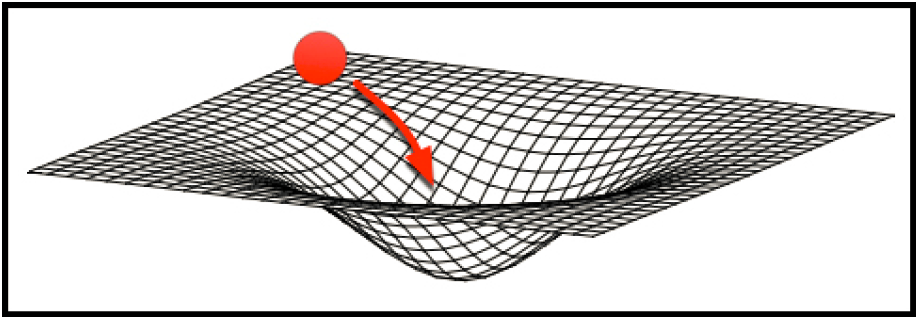
\includegraphics[scale=0.4]{Arda_1.png}
    \caption[Arda 1]{Esempio di attrazione gravitazionale}
    \label{etichetta}
    \end{center}
\end{figure}

\subsubsection{Generazione del modello}
La metafora legata alla fisica gravitazionale \`e probabilmente quella pi\`u intuitiva
per questo modello astratto di previsione della traiettoria.
Da notare che anche altre leggi fisiche, quali la diffusione del suono e i campi magnerici ,
hanno modelli fisici simili a quelli gravitazionali. Questi ultimi infatti possono essere
particolarmente interessanti poich\'e prevedono la presenza sia di potenziali negativi
che esercitano forze attrattive (per oggetti di carica positiva) come quelle dei
campi gravitazionali, sia di potenziali positivi generati dalla presenza di cariche
positive che esercitano forze repulsive (per oggetti di carica positiva), come
illustrato in Figura 1.3.\\
L'introduzione di forze repulsive nel nostro modello pu\`o sembrare inutile, ma analizzando
bene il concetto di repulsivit\`a possiamo fruttarlo in casi particoli. Un esempio pu\`o
essere l'indicare zone che non posso essere raggiunte oppure oltrepassate per via di limiti
fisici o strutturali come ad esempio il passaggio in mare o attreverso fiumi, montagne o edifici.
In questi casi la traiettoria dovr\`a essere deviata per non incorrete in tragitti fisicamente
impossibi e/o non veritieri. Ci sono anche casi pi\`u sottili, come divieti di transito o
zone ad acesso limitato, che, seppur non limitate per ostruzioni naturali o fisiche, rimangono
sempre zone da evitare in un possibile calcolo del destinazione.

\begin{figure}
\begin{center}
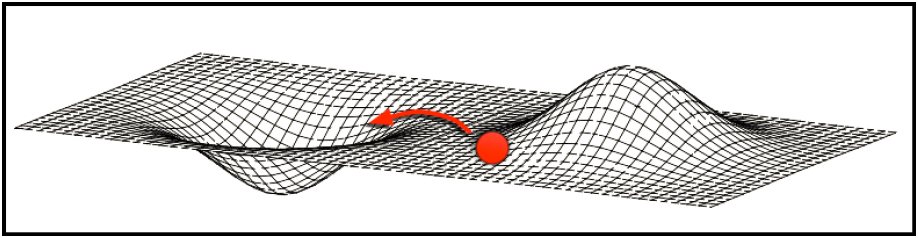
\includegraphics[scale=0.4]{Arda_2.png}
\caption[Arda 2]{Arda: Esempio di attrazione e repulsione gravitazionale}
\label{etichetta}
\end{center}
\end{figure}

Come si pu\`o notare, in questo tipo di modello fisico, basato sui campi
elettrici, \`e pi\`u semplice ragionare in termini di potenziale presente in una
certa localit\`a piuttosto che di presenza di una certa carica nella localit\`a stessa.
Inoltre, l'analisi delle abitudini di un utente dar\`a come risultato un valore di
importanza da assegnare a ciascuna delle localit\`a prese in considerazione e
potrebbe non essere banale scegliere un piccolo insieme di punti di interesse
disposti sulla superficie. Si pu\`o quindi scegliere di interpretare i valori
di importanza, assegnati a ciascuna localit\`a, come i valori opposti del potenziale
elettrico presente in quella data localit\`a. In tal modo, maggiore \`e l'importanza,
minore \`e il valore del potenziale e quindi maggiore \`e l'attrazione esercitata dalla localit\`a.

\subsection{ARDA}
Dopo aver fatto le dovute premesse, possiamo descrivere l'algoritmo di previsione
basato sul modello astratto precedentemente descritto nel paragrafo 1.2.2.
In questo paragrafo vengono introdotte le formule utilizzate per eseguire una previsione
della traiettoria dell'utente, sia a breve termine che a lungo termine, sulla base
dei valori di importanza assegnati alle localit\`a secondo un dato indice di stima.
Le simulazioni fisiche descritte vengono effettuate in uno spazio bidimensionale
a valori continui rappresentante l'area di interesse. Poich\'e i dati ottenuti
dall'analisi degli spostamenti degli utenti sono relativi ad un insieme
discreto di localit\`a, il piano utilizzato nella simulazione deve essere
suddiviso in sezione di ugual dimensione. Durante la simulazione, l'applicazione
delle forze in gioco previste dal modello astratto viene operata in modo omogeneo
a tutti i punti del piano continuo appartenenti ad una stessa sezione della griglia,
ovvero a tutti i punti dello spazio appartenenti ad una stessa localit\`a.
Si suppone che i valori di importanza utilizzati siano disponibili per mezzo
di una struttura dati di tipo matriciale $M_{imp}$ che rappresenti la griglia delle
localit\`a.

\subsubsection{Utilizzo dei valori di importanza}
Utilizzando un modello gravitazionale, possiamo definire una matrice $M_{pot}$ che
rappresentanti l'energia potenziale elettrica di ciascuna localit\`a. Ciascun ODP
sar\`a attratto dalle aree a basso potenziale, associate con le localit\`a pi\`u
importanti per l'individuo.
Per definire i valori di $M_{pot}$ \`e possibile utilizzare qualsiasi indice di
localit\`a gi\`a indicati in precedenza:
\begin{itemize}
\item $\sharp$\textit{visits}: il numero di volte in cui l'utente \`e stato nella localit\`a;
\item \textit{avgTime}: il tempo medio delle visite effettuate dall'utente nella localit\`a;
\item \text{totTime}: il tempo totale passato dall'utente nella localit\`a durante le sue
visite;
\item \textit{spaceRank}: basato su un'analisi dello storico degli spostamenti dell'utente
e sull'analisi dell'intorno di ciascuna localit\`a.
\end{itemize}
Al di la degli indici adottati per l'analisi del territorio, importante e comprendere
come il risultato di tale procedura sia una matrice di importanza
$M_{imp}$, che associa i valori pi\`u alti alle localit\`a dalla maggiore importanza.
Dato che il nostro modello fisico utilizza valori di importanza opposti, dobbiamo
generare partendo da $M_{imp}$ la matrice a valori opposti $M_{pot}$, rappresentante il
potenziale delle locazioni. Per ottenere ci\`o si \`e scelto di utilizzare la funzione
$f(x)=-x$, ma sarebbe stato possibile adottare anche funzioni di tipo
polinomiale, logaritmico od esponenziale. A questo punto non rimane altro che
calcolare la matrice delle accelerazioni $M_{acc}$ dipendenti dalla matrice $M_{pot}$
appena calcolata. In particolare ogni cella conterr\`a il vettore accelerazione relativo
alla localit\`a rappresentata dalla cella della matrice. $M_{acc}$ \`e dunque calcolato
utilizzando il gradiente:
\begin{equation}
M_{acc} = - \vec{\bigtriangledown}(M_{pot})
\end{equation}
Come ultimo passaggio andiamo a normalizzare i vettori di accelerazione ottenuti in $M_{acc}$
in modo che la media delle accelerazioni rilevate nei dati acquisiti corrisponda
alla media delle accelerazioni contenute in $M_{acc}$.
Per fare ci\`o \`e opportuno seguire la seguente procedura:
\begin{enumerate}
\item Rilevare tutte le magnitudo dei vettori di accelerazione dai dati acquisiti
e calcolarne il valore medio: \textit{AvgRealMagnitude}
\item Rilevare tutte le magnitudo dei vettori di accelerazione di Macc e calcolarne
il valore medio: \textit{AvgMaccMagnitude}
\item Per ogni vettore accelerazione diMacc moltiplicare gli elementi del vettore
per la costante ricavata da $\frac{AvgRealMagnitude}{AvgMaccMagnitude}$
\end{enumerate}

\begin{figure}
\begin{center}
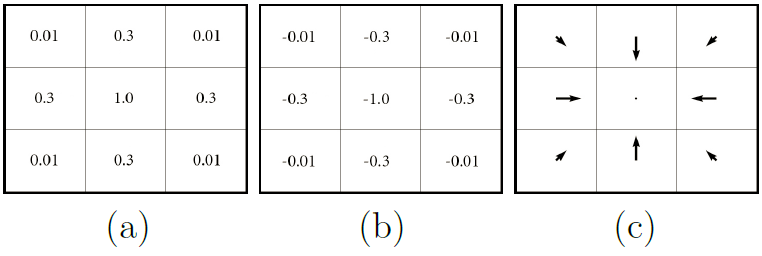
\includegraphics[scale=0.4]{forze.png}
\caption[Arda 2]{(a) Valori di importanza assegnati alle localita $M_{imp}$;(b) valori di potenziale assegnati alle localita $M_{pot}$;(c) vettori
di accelerazione $M_{acc}$}
\label{etichetta}
\end{center}
\end{figure}

\subsubsection{Calcolo della traiettoria futura}
Dopo aver calcolato e impostato l'importanza per ogni localit\`a, si pu\`o procedere
al calcolo della previsione della traiettoria utilizzando:
\begin{itemize}
\item Un tempo di campionamento, indicante la profondit\`a temporale in secondi
della singola previsione. Nelle nostre rilevazioni abbiamo utilizzato $\bigtriangleup_{t} = 1$
\item La posizione $(x_{1}; y_{1})$ al tempo corrente $t_{1}$
\item La posizione $(x_{0}; y_{0})$ al tempo $t_{0} = t_{1} - \bigtriangleup_{t}$
\item La matrice di accelerazione $M_{acc}$, dove $M_{acc}[x,y]$ contiene il vettore di
accelerazione per la localit\`a (x, y)
\item Una funzione frenante $\gamma(M_{imp},x,y)$, che ritorni il fattore frenante in base
all'importanza della localit\`a
\end{itemize}
Quest'ultima funzione viene proposta per migliorare l'iterazione tra l'ODP e le
forze attrattive delle localit\`a mi maggiorn interesse. Infatti le localit\`a
poco importanti o con forza repulsiva giustamente respingono l'ODP in modo non
passi in quelle zone, ma le localit\`a di maggior interesse devono avere un'ulteriore
forza che permetta all'ODP di rallentare l'avanzamento fino anche a firmarlo.
Nel nostro caso abbiamo adottato una funzione frenante che garantisse
fattori frenanti che andassero dal 1.5\% al 10\% del valore ad ogni previsione,
a seconda dell'importanza della localit\`a percorsa. Tale decisione ha dunque
portato alla definizione della seguente funzione:
\begin{equation}
    \gamma(M_{imp},x,y) = 0.015 + 0.085 \times M_{imp}[x,y]
\end{equation}
Una volta definiti i vari elementi del processo previsionale, non rimane che
proporre la formula adottata per simulare l'itinerario dell'ODP e quindi per
prevedere la posizione $(x_{2},y_{2})$ dell'utente al tempo $t_{2} = t_{1} +\bigtriangleup_{t}$.
Tale funzione \`e la Verlet integration formula:
\begin{equation}
\begin{matrix}
(x2; y2) = & \left \{ [2 - \gamma(M_{imp},x_{1},y_{1})] \times (x_{1},y_{1}) \right \}\\
 & - \left \{ [1 - \gamma(M_{imp},x_{1},y_{1})] \times (x_{0},y_{0}) \right \} \\
 & + \left \{ M_{acc}[x,y] \times \bigtriangleup_{t}^{2} \right \}
\end{matrix}
\end{equation}
Tale formula pu\`o essere applicata iterativamente per calcolare le future
posizioni dell'ODP in ogni tempo $t_{k} = t_{1} + (k - 1) \times \bigtriangleup_{t}$, con $k \geq 2$ .

\subsubsection{Utilizzo di informazioni aggiuntive}
L'algoritmo descritto prevede l'utilizzo della matrice $M_{imp}$ costruita in base ai
valori di importanza ottenuti dall'analisi dei comportamento dell'utente durante
il periodo di osservazione. Tuttavia,il modello astratto prevede l'utilizzo
di informazioni sull'importanza delle localit\`a indipendentemente dalla fonte di
tali dati.\\
Come suggerito dalla precedente tesi, per poter migliorare la previsione delle traiettorie
si potrebbero valutare anche altri valori al di fuori degli indici di importanza.
Uno su tutti potrebbe essere l'arco temporale in cui svolgo la simulazione.
Eseguire la simulazione di uno spostamente durante la settimana potrebbe essere abbastanza
preciso visto che quasi tutte le persone lavorano in un luogo fisso e vi restano in una determinata
fascia oraria. Lo stesso test eseguito in uno spostamente nel weekend darebbe risultati sfalsati perch\`e
si avrebbe il luogo di lavoro come localit\`a di interesse. Dividere le simulazioni
per giorno delle settimana potrebbe comportare un notevole miglioramente sia dell'analisi
dell'importanza delle localit\`a, sia del calcolo della destinazione.
Allo stesso modo \`e potremmo utilizzare altre tipologie di dati non strettamente legate
agli spostamenti ma che possono essere integrate in questo algoritmo e
sfruttate in alcune particolari situazioni come gli impegni in una calendario
(sfruttando l'orario e il luogo dell'appuntamento) oppure
da reti sociali (controllando il posizionamento di amici, colleghi o eventi a cui abbiamo aderito).
La flessibilit\`a del modello nella codifica dei dati da utilizzare come informazioni
sull'importanza delle localit\`a viene sottolineata dalla semplicit\`a con
la quale le diverse tipologie di dati possono essere integrate in un'unica valutazione.
Due o pi\`u fonti di dati possono infatti essere sovrapposte, mediante una
combinazione lineare delle matrici di importanza relative alle singole fonti, generando un'unica matrice:
\begin{equation}
M_{imp} = \alpha_{1}M_{fonte1} + \alpha_{2}M_{fonte2} + \dots
\end{equation}
dove $\alpha_{1}M_{fonte1} + \alpha_{2}M_{fonte2} + \dots$ sono le matrici relative
alle singole fonti ed $\alpha_{1},\alpha_{2},\dots$
sono i rispettivi pesi utilizzati per la combinazione lineare.
